\documentclass[12pt, a4paper]{article}

% ── 中文支持 ──────────────────────────────────────────────
\usepackage{ctex}

% ── 页面设置 ──────────────────────────────────────────────
\usepackage[top=2.5cm, bottom=2.5cm, left=3cm, right=3cm]{geometry}

% ── 图表 ──────────────────────────────────────────────────
\usepackage{graphicx}
\usepackage{caption}
\usepackage{float}
\usepackage{booktabs}
\usepackage{array}

% ── 数学 ──────────────────────────────────────────────────
\usepackage{amsmath}

% ── 代码块 ────────────────────────────────────────────────
\usepackage{listings}
\usepackage{xcolor}
\lstset{
  basicstyle=\ttfamily\small,
  backgroundcolor=\color{gray!10},
  frame=single,
  breaklines=true,
  columns=flexible
}

% ── 超链接 ────────────────────────────────────────────────
\usepackage{hyperref}
\hypersetup{colorlinks=true, linkcolor=blue, citecolor=blue}

% ── 页眉页脚 ──────────────────────────────────────────────
\usepackage{fancyhdr}
\pagestyle{fancy}
\fancyhf{}
\rhead{AI for Chemistry --- HW6}
\lhead{Au 神经网络势函数训练报告}
\cfoot{\thepage}

% ─────────────────────────────────────────────────────────
\begin{document}

% ── 封面 ──────────────────────────────────────────────────
\begin{titlepage}
  \centering
  \vspace*{3cm}
  {\LARGE\bfseries Au 神经网络势函数训练报告\par}
  \vspace{0.5cm}
  {\large 基于 LASP 软件的全局神经网络势（G-NNP）训练\par}
  \vspace{2cm}
  \begin{tabular}{rl}
    \textbf{软件版本} & LASP 3.7.3 (NN single-precision) \\[4pt]
    \textbf{元素体系} & Au（金，单元素） \\[4pt]
    \textbf{训练日期} & 2026年5月22日 \\[4pt]
    \textbf{耗时}     & 36 分 58 秒（4 核并行） \\
  \end{tabular}
  \vfill
  {\small 参考文献：Huang et al., \textit{Chem. Sci.} 2017, 8, 6327;\quad
          Huang et al., \textit{Chem. Sci.} 2018, 9, 8644.}
\end{titlepage}

% ── 正文 ──────────────────────────────────────────────────
\section{任务概述}

本次计算使用 LASP（Large-scale Atomic Simulation with neural network Potential）
软件，对 Au 元素训练一套全局神经网络势函数（Global Neural Network Potential，G-NNP）。
训练完成后得到的势函数文件为 \texttt{Au.pot}，可用于后续的结构搜索（SSW）、
分子动力学（MD）等模拟任务。

\subsection{\texttt{lasp.in} 关键参数}

\begin{lstlisting}
explore_type  train       % 任务类型：势函数训练
Jobname       Au          % 作业名，对应 Au.input 和输出 Au.pot
NNepochs      1000        % 最大训练步数（L-BFGS 迭代）
Ntrain        1037        % 训练集结构数量
OutpotFreq    200         % 每 200 步保存一次势函数至 SavePot/
Nparabfgs     4           % 4 核并行更新 L-BFGS Hessian
Histbfgs      100         % L-BFGS 历史向量数
\end{lstlisting}

\section{神经网络结构}

使用全连接前馈神经网络（Fully-Connected Feed-Forward NN），以
\textbf{幂型结构描述符（PTSD，Power-Type Structural Descriptor）}作为输入，
输出每个 Au 原子的原子能量，加和得到体系总能量。

\subsection{网络层次}

\begin{table}[H]
  \centering
  \caption{Au NNP 网络架构}
  \begin{tabular}{cccc}
    \toprule
    层编号 & 类型 & 节点数 & 激活函数 \\
    \midrule
    1 & 输入层（PTSD 描述符） & 72 & --- \\
    2 & 全连接隐藏层          & 80 & tanh（类型 2） \\
    3 & 全连接隐藏层          & 48 & cos（类型 24） \\
    4 & 输出层（原子能量）    &  1 & 线性（类型 0） \\
    \bottomrule
  \end{tabular}
\end{table}

网络总参数量：\textbf{9777 个}。

\subsection{输入描述符（PTSD）}

输入层共 72 维，由以下对称函数组成：

\begin{table}[H]
  \centering
  \caption{PTSD 描述符构成}
  \begin{tabular}{lcc}
    \toprule
    描述符类型 & 物理含义 & 维数 \\
    \midrule
    S1（KS1 两体）  & 径向分布，$\sum r_{ij}^n f_c(r_{ij})$         & 22 \\
    S2（KS2 两体）  & Q值两体描述符                                  & 17 \\
    S3（两体）      & 两体扩展                                       &  7 \\
    S4（两体）      & 两体扩展                                       &  8 \\
    S5（三体）      & 角度依赖三体描述符                             &  8 \\
    S6（三体）      & 角度依赖三体描述符                             &  6 \\
    S7（三体）      & 三体扩展                                       &  4 \\
    \midrule
    合计            &                                                & 72 \\
    \bottomrule
  \end{tabular}
\end{table}

\section{训练过程}

\subsection{优化方法}

采用 \textbf{L-BFGS（Limited-memory Broyden–Fletcher–Goldfarb–Shanno）}
二阶优化算法，共训练 1000 步。损失函数定义为：

\begin{equation}
  C = C_e + C_f + C_s
\end{equation}

其中 $C_e$、$C_f$、$C_s$ 分别为能量项、力项和应力项的均方误差加权和。

\subsection{训练集}

训练集包含 \textbf{1037 个 Au 结构}（来自 \texttt{TrainStr.txt}），
涵盖团簇、块体等多种构型，能量、力及应力标签由第一性原理计算提供。

\subsection{损失函数收敛曲线}

图~\ref{fig:loss} 展示了训练过程中各损失项及精度指标随训练步数的变化。

\begin{figure}[H]
  \centering
  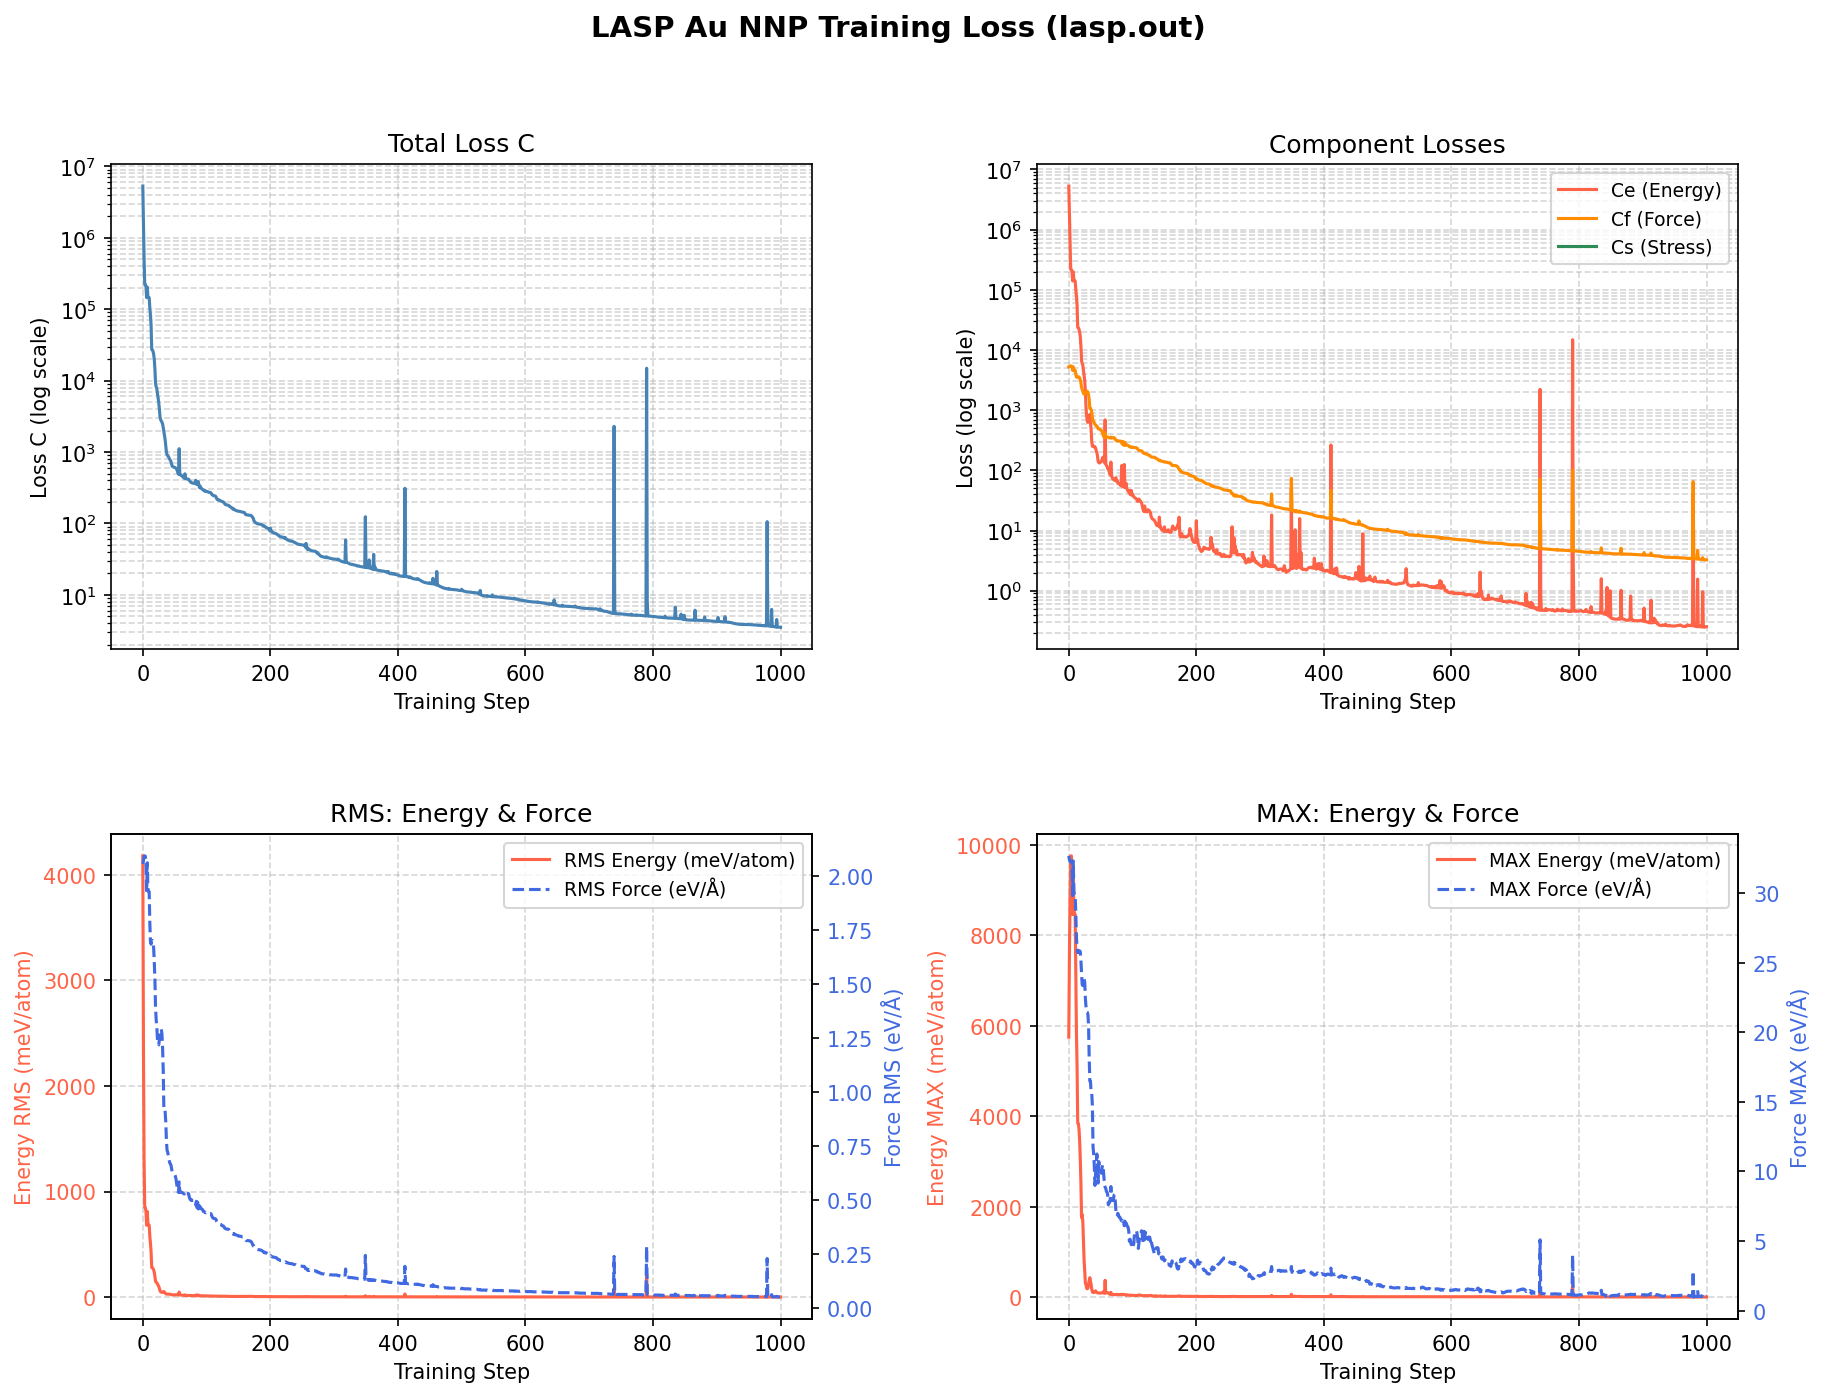
\includegraphics[width=\textwidth]{training_loss.png}
  \caption{Au NNP 训练损失曲线。
    左上：总损失 $C$（对数坐标）；
    右上：各分量损失 $C_e$（能量）与 $C_f$（力）；
    左下：能量与力的 RMS 误差（双 Y 轴）；
    右下：能量与力的 MAX 误差（双 Y 轴）。}
  \label{fig:loss}
\end{figure}

初始步（step 0）与最终步（step 1000）的关键指标对比如表~\ref{tab:convergence} 所示。

\begin{table}[H]
  \centering
  \caption{训练初末关键指标对比}
  \label{tab:convergence}
  \begin{tabular}{lccc}
    \toprule
    指标 & 初始（step 0） & 最终（step 1000） & 降低倍数 \\
    \midrule
    总损失 $C$                 & 5{,}288{,}616  & 3.509             & $\sim 1.5\times10^6$ \\
    RMS 能量 (meV/atom)        & 4179.2         & 0.915             & $\sim 4566$ \\
    RMS 力 (eV/\AA)            & 2.057          & 0.051             & $\sim 40$ \\
    RMS 应力 (GPa)             & 1.558          & 0.007             & $\sim 223$ \\
    \bottomrule
  \end{tabular}
\end{table}

\section{最终势函数精度}

训练完成后，\texttt{Au.pot} 记录的最终拟合精度如表~\ref{tab:accuracy} 所示。

\begin{table}[H]
  \centering
  \caption{Au.pot 最终拟合精度}
  \label{tab:accuracy}
  \begin{tabular}{lccc}
    \toprule
    误差类型 & 能量 (meV/atom) & 力 (eV/\AA) & 应力 (GPa) \\
    \midrule
    RMS & 0.915 & 0.051 & 0.007 \\
    MAX & 3.898 & 1.061 & 0.066 \\
    \bottomrule
  \end{tabular}
\end{table}

能量 RMS 误差为 \textbf{0.915 meV/atom}，远低于化学精度阈值（$\sim$1 kcal/mol
$\approx$ 43 meV/atom），表明训练得到的势函数具有很高的准确性，
可以可靠地用于 Au 体系的后续模拟。

\section{输出文件说明}

\begin{table}[H]
  \centering
  \caption{主要输出文件}
  \begin{tabular}{ll}
    \toprule
    文件 & 说明 \\
    \midrule
    \texttt{Au.pot}              & 训练完成的神经网络势函数（最终 step 1000） \\
    \texttt{lasp.out}            & 训练日志，包含每步损失、RMS/MAX 误差 \\
    \texttt{SavePot/pot\_in\_step-*} & 每 200 步保存的中间势函数快照 \\
    \texttt{training\_loss.png}  & 损失曲线可视化图（由 \texttt{plot\_loss.py} 生成） \\
    \texttt{TrainStr.txt}        & 1037 个训练结构（LASP 格式） \\
    \texttt{TrainFor.txt}        & 对应的力标签 \\
    \bottomrule
  \end{tabular}
\end{table}

\section{结论}

本次训练成功得到了 Au 元素的神经网络势函数。经过 1000 步 L-BFGS 优化，
总损失从初始的 $5.3\times10^6$ 降低至 $3.5$，能量 RMS 误差从 4179 meV/atom
降低至 \textbf{0.915 meV/atom}，达到了接近第一性原理的精度水平。
该势函数后续可直接用于 Au 团簇或块体的 SSW 全局结构搜索、
分子动力学模拟等高通量计算任务。

\end{document}
